% Latex template: mahmoud.s.fahmy@students.kasralainy.edu.eg
% For more details: https://www.sharelatex.com/learn/Beamer

\documentclass{beamer}          % Document class

\usepackage[french]{babel}        % Set language
\usepackage[utf8x]{inputenc}      % Set encoding
\usepackage{verbatim}      % Set encoding
\usepackage[normalem]{ulem}

\mode<presentation>            % Set options
{
  \usetheme{default}          % Set theme
  \usecolortheme{default}         % Set colors
  \usefonttheme{default}          % Set font theme
  \setbeamertemplate{caption}[numbered]  % Set caption to be numbered
}

% Uncomment this to have the outline at the beginning of each section highlighted.
%\AtBeginSection[]
%{
%  \begin{frame}{Outline}
%  \tableofcontents[currentsection]
%  \end{frame}
%}

\usepackage{graphicx}          % For including figures
\usepackage{booktabs}          % For table rules
\usepackage{hyperref}          % For cross-referencing

\title{LRGrep}  % Presentation title
\subtitle{Expliquer les erreurs d'un analyseur LR}
\author{Frédéric Bour}                % Presentation author
\institute{Tarides, Inria}          % Author affiliation
\date{30 mars 2023}                  % Today's date

\begin{document}

% Title page
% This page includes the informations defined earlier including title, author/s, affiliation/s and the date
\begin{frame}
  \titlepage
\end{frame}

% Outline
% This page includes the outline (Table of content) of the presentation. All sections and subsections will appear in the outline by default.
\begin{frame}{Plan}
  \tableofcontents
\end{frame}

\AtBeginSection[]{
  \begin{frame}
  \vfill
  \centering
  \begin{beamercolorbox}[sep=8pt,center,shadow=true,rounded=true]{title}
    \usebeamerfont{title}\insertsectionhead\par%
  \end{beamercolorbox}
  \vfill
  \end{frame}
}

\section{Introduction}

\newcommand\pro{\item[$+$]}
\newcommand\con{\item[$-$]}

\begin{frame}{Les analyseurs LR}

  \begin{itemize}
    \pro \textbf{Déclaratif} \\
         {\small Travaille sur une spécification de la grammaire.}
    \pro \textbf{Efficace} \\
         {\small Reconnaissance en $O(n)$.}
    \pro \textbf{Non-ambigu} \\
         {\small Absence d'ambiguité décidable statiquement.}
    \pause
    \con \textbf{Expressivité limitée} \\
         {\small Certains langages ne sont pas LR.}
    \con \textbf{Grammaire pas naturelle} \\
         {\small Il peut exister une grammaire LR, mais difficile de la trouver.}
         %{\small Certains langages sont difficilement LR !}
    \con \textbf{Difficulté à gérer les erreurs} \\
         {\small On peut situer le problème mais pas l'expliquer.}
  \end{itemize}

\end{frame}

\begin{frame}[fragile]{Pratiques \& état de l'art (1/2)}
  \begin{itemize}
    \item Bison \& Yacc (Johnson, 1975)
      \begin{itemize}
      \item On rajoute des règles pour les cas incorrects
      \item Une forme d'{\em exception}: le {\em token} \textbf{error}
      \end{itemize}
  \end{itemize}
\pause
\small
\begin{verbatim}
| LPAREN seq_expr error
    { unclosed "(" $loc($1) ")" $loc($3) }
\end{verbatim}
\pause
\begin{verbatim}
$ more foo.ml
(2 + )
$ ocamlc -c foo.ml
File "foo.ml", line 1, characters 5-6:
1 | (2 + )
         ^
Error: Syntax error: ')' expected
File "foo.ml", line 1, characters 0-1:
1 | (2 + )
    ^
This '(' might be unmatched
\end{verbatim}
\end{frame}

\begin{frame}{Pratiques \& état de l'art (2/2)}
  \begin{itemize}
    \item Merr (Jeffery 2003)
      \begin{itemize}
        \item À partir d'exemples, on associe un message d'erreur à un état
      \end{itemize}
    \pause
    \item Menhir (Pottier 2016)
      \begin{itemize}
        \item Énumération d'exemples couvrant tous les états d'erreur
        \item On peut contrôler les réductions \only<3>{{\em ``(1 + 2''}}
        \item Application industrielle d'envergure (CompCert)
      \end{itemize}
    \pause
    \pause
    \item Menhir': {\em Faster reachability analysis for LR(1) parsers} (Bour \& Pottier, 2021)
      \begin{itemize}
        \item Accélère l'énumération par un facteur 100 à 1000
      \end{itemize}
  \end{itemize}
\end{frame}

\begin{frame}{Objectif}

  Augmenter une grammaire LR avec une spécification des messages d'erreur qui soit :
  \begin{itemize}
    \item Déclarative
      % Bison, Merr, Menhir, ...
      % Un langage spécifique auquel on peut donner plusieurs interprétations :
      % opérationnelle pour produire des messages d'erreur à l'exécution
      % statique, pour décider de la couverture, du code mort
    \item Expressive (\& concise)
      % Contrairement à Merr et Menhir.
      % Factoriser des cas communs
      % Pour se référer à des éléments grammaticaux comme Bison
    \item Maintenable
      % Contrairement à Merr et Menhir.
    \item Séparée de la grammaire
      % Contrairement à Bison
  \end{itemize}
\end{frame}

\section{Intégration à Menhir \& démonstration}

\begin{frame}{Intégration à un analyseur Menhir}

  \begin{itemize}
    \item Fichiers :
      \begin{itemize}
      \item Grammaire, extension \texttt{.mly}
      \item<2-> Spécification des erreurs, \texttt{.mlyl}
      \end{itemize}
    \item Compilation :
      \begin{itemize}
        \item Menhir traite le \texttt{.mly} et produit un analyseur syntaxique
        \item<2-> LRgrep traite le \texttt{.mlyl} et produit un analyseur d'erreur
      \end{itemize}
    \item Exécution :
      \begin{itemize}
        \item L'analyseur syntaxique traite une entrée
        \item En cas de succès : il renvoie un AST (une valeur sémantique)
        \item En cas d'échec : il lance une exception \\
        \uncover<2->{
        \item L'analyseur d'erreur attrape l'exception, puis \\
            inspecte l'état de l'analyseur syntaxique \\
            ($\approx$ débogueur et \texttt{coredump})
        }
      \end{itemize}
  \end{itemize}

\end{frame}

% \begin{frame}[fragile]{Spécification des erreurs}
%   Le fichier \texttt{.mlyl} a la même structure qu'un fichier \texttt{ocamllex} : \\
%   \begin{itemize}
%     \item une ou plusieurs règles composées d'une liste de clauses
%     \item chaque clause est un motif accompagné d'une action sémantique.
%   \end{itemize}
%
%   \pause
%
%   \begin{block}{Exemple: clause d'une parenthèse non fermée}
%     \begin{verbatim}
% | lp=LPAREN; [_* / . RPAREN]
%   { "Unclosed parenthesis at " ^ print_loc $startloc(lp) }
%   \end{verbatim}
%   \end{block}
% \end{frame}

\begin{frame}{Application à OCaml}
  Action !
\end{frame}

\section{Théorie et concepts de LRgrep}

\begin{frame}{Caractériser les erreurs: complémentaire}
  Une grammaire $G$ dénote un langage $L$, un sous-ensemble des mots sur un alphabet $\Sigma$ (aussi appelé ensemble des terminaux).
  $$
  [\![G\,]\!] = L \subset \Sigma^*
  $$

  \pause
  A priori, une entrée erronée est n'importe quel mot qui n'appartient pas au langage :
  $$
  \Sigma^* / L
  $$

  \pause
  La grammaire donne aussi de la structure aux mots: les dérivations grammaticales.
  \\
  Quelle structure peut-on donner aux erreurs ?
\end{frame}

\begin{frame}{Caractériser les erreurs: le front d'erreur}
  Un analyseur LR reconnaît l'entrée de gauche à droite et échoue dès que l'entrée n'est préfixe d'aucun mot du langage (c'est-à-dire le plus tôt possible, c'est la {\em propriété du préfixe viable}).

  % Attention aux conflits cependant !
  % C'est grâce à ça qu'on peut raporter au moins la position de l'erreur.

  \pause
  Considérons l'ensemble de ces entrées erronées et minimales :
  $$
  \mathcal E_L = \left\{ (u, t) \in \Sigma^*\times\Sigma\ \big|\
    \vext{viable}(u) \wedge \neg \vext{viable}(u.t)
  \right\} \\
  \qquad \text{avec} \text{viable}(u) = \exists v \in \Sigma^*,\ u.v \in L
  $$
  \pause
  \\ \ \\
  Les $u$ sont des préfixes valides et les $t$ sont les premiers terminaux
  à faire échouer l'analyse.

\end{frame}

%\begin{frame}{}
  %\begin{block}
%{Intuition sur les analyseurs << Shift-Reduce >>}
%Comment interpréter la pile d'un analyseur?
  %\end{block}
%\end{frame}

\begin{frame}[t]{Caractériser les erreurs: régularisation}

 \  \\
 \

  Comme les $u$ sont valides, on peut les donner comme une entrée partielle à l'automate LR et récupérer une pile. On note cette opération $\text{im}$, et on construit :

  $$
  \mathcal E_G = \left\{\ (\text{im}(u), t)\ \mid\ (u, t) \in \mathcal E_L\ \right\}
  $$

  \pause
  \begin{block}{Théorème (Aho \& Ullman, 1972)}
  %L'ensemble des \only<3->\sout{préfixes viables des formes sententielles droites
  %d'une grammaire}\only<3->{ \textbf{piles d'un automate LR}} est un langage régulier. \\
  L'ensemble des \only<-2>{{\em préfixes viables des formes sententielles droites
  d'une grammaire}}\only<3->{\textbf{piles d'un automate LR}} est un langage régulier. \only<3->{ \\ \ } \\
  \end{block}

  \pause
  \pause

  Donc $\mathcal E_G$ est un ensemble régulier (rationnel)!

  \textbf{Bonne nouvelle:} de nombreuses propriétés sont décidables, on
  a une boîte à outil riche pour analyser ces ensembles (les expressions
  rationnelles).

\end{frame}

\begin{frame}{Intuition sur les analyseurs << Shift-Reduce >>}

  L'analyse {\em bottom-up} se fait avec une pile:
  \begin{itemize}
    \item on consomme l'entrée de gauche à droite ({\em push})
    \item on construit la dérivation en partant des feuilles,
          que l'on enracine progressivement ({\em pop} feuilles, {\em push} noeud)
    \item la pile sauvegarde les dérivations intermédiaires
    \item l'analyse se termine avec la racine de la dérivation sur la pile
  \end{itemize}

  \pause

  Exemple avec une grammaire minimaliste:
  $$
  \begin{array}{rl}
    exp ::= & num \\
          | & exp + exp \text{, associatif à droite}\\
  \end{array}
  $$

  On va analyser l'expression $1+2+3$.
\end{frame}

\begin{frame}[t]{Intuition sur les analyseurs << Shift-Reduce >>}
  \begin{columns}[T]
    \begin{column}{.5\textwidth}
    \scalebox{0.8}{
      \begin{tabular}{|l|l|}
        \hline
        Pile & Entrée \\
        \hline
        $\emptyset$ & \texttt{num + num + num \$} \\
        \uncover<3->{\texttt{\only<4>{\underline}{num}}
                                              & \texttt{+ num + num \$}} \\
        \uncover<5->{\texttt{exp}             & \texttt{+ num + num \$}} \\
        \uncover<6->{\texttt{exp +}           & \texttt{num + num \$}} \\
        \uncover<7->{\texttt{exp + \only<8>{\underline}{num}}
                                              & \texttt{+ num \$}} \\
        \uncover<9->{\texttt{exp + exp}       & \texttt{+ num \$}} \\
        \uncover<10->{\texttt{exp + exp +}    & \texttt{num \$}} \\
        \uncover<11->{\texttt{exp + exp + \only<12>{\underline}{num}} & \texttt{\$}} \\
        \uncover<13->{\texttt{exp + \only<14>{\underline}{exp + exp}} & \texttt{\$}} \\
        \uncover<15->{\texttt{\only<16>{\underline}{exp + exp}}       & \texttt{\$}} \\
        \uncover<17->{\texttt{exp}             & \texttt{\$}} \\
        \uncover<18->{\texttt{exp \$}          & $\emptyset$} \\
        \uncover<19->{\texttt{but}             & $\emptyset$} \\
        \hline
      \end{tabular}
    }
    \end{column}

    \begin{column}{.5\textwidth}
    \vspace{-10pt}
    \only<1-2>{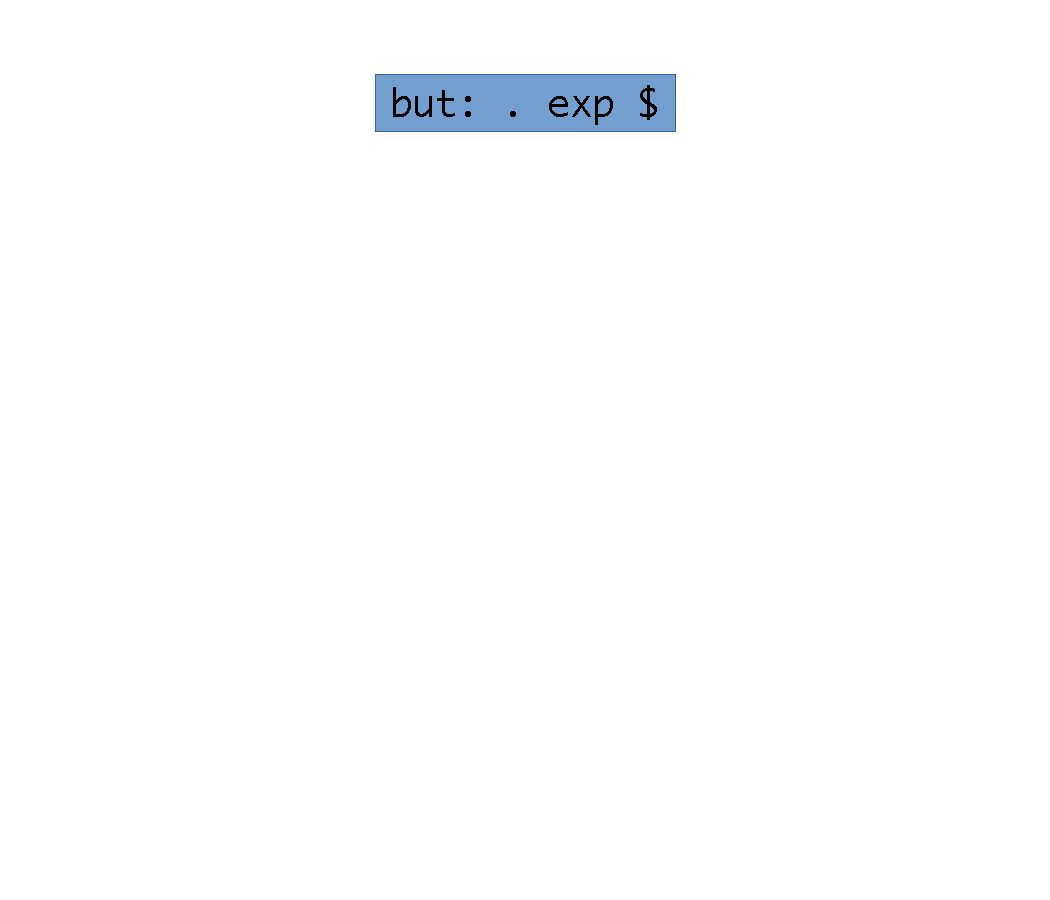
\includegraphics[page=1,width=160pt]{dfa.fr.pdf}}
    \only<3>{\includegraphics[page=2,width=160pt]{dfa.fr.pdf}}
    \only<4>{\includegraphics[page=3,width=160pt]{dfa.fr.pdf}}
    \only<5>{\includegraphics[page=4,width=160pt]{dfa.fr.pdf}}
    \only<6>{\includegraphics[page=5,width=160pt]{dfa.fr.pdf}}
    \only<7>{\includegraphics[page=6,width=160pt]{dfa.fr.pdf}}
    \only<8>{\includegraphics[page=7,width=160pt]{dfa.fr.pdf}}
    \only<9>{\includegraphics[page=8,width=160pt]{dfa.fr.pdf}}
    \only<10>{\includegraphics[page=9,width=160pt]{dfa.fr.pdf}}
    \only<11>{\includegraphics[page=10,width=160pt]{dfa.fr.pdf}}
    \only<12>{\includegraphics[page=9,width=160pt]{dfa.fr.pdf}}
    \only<13>{\includegraphics[page=11,width=160pt]{dfa.fr.pdf}}
    \only<14>{\includegraphics[page=9,width=160pt]{dfa.fr.pdf}}
    \only<15>{\includegraphics[page=11,width=160pt]{dfa.fr.pdf}}
    \only<16>{\includegraphics[page=13,width=160pt]{dfa.fr.pdf}}
    \only<17>{\includegraphics[page=14,width=160pt]{dfa.fr.pdf}}
    \only<18>{\includegraphics[page=15,width=160pt]{dfa.fr.pdf}}
    \only<19>{\includegraphics[page=16,width=160pt]{dfa.fr.pdf}}
    %
    %\only<1,2,8,12,14,16>{\uncover<0>{X}}%
    \only<3>{Shift \texttt{num}}%
    \only<4-5>{Reduce \texttt{exp: num}}%
    \only<6>{Shift \texttt{+}}%
    \only<7>{Shift \texttt{num}}%
    \only<8-9>{Reduce \texttt{exp: num}}%
    \only<10>{Shift \texttt{+}}%
    \only<11>{Shift \texttt{num}}%
    \only<12-13>{Reduce \texttt{exp: num}}%
    \only<14-15>{Reduce \texttt{exp: exp + exp}}%
    \only<16-17>{Reduce \texttt{exp: exp + exp}}%
    \only<18>{Shift \texttt{\$}}%
    \only<19>{Reduce \texttt{but: exp \$}}%

    \texttt{\\
    \only<1-2>{but: . exp \$}
    \only<2>{
      \rule{\textwidth}{0.5pt}
      exp: . num \\
      exp: . exp + exp
    }
    \only<3,7,11>{%
      exp: num .
    }
    \only<5>{%
      but: exp . \$ \\
      exp: exp . + exp
    }
    \only<6,10>{%
      exp: exp + . exp
      \rule{\textwidth}{0.5pt}
      exp: . num \\
      exp: . exp + exp
    }
    \only<9,13-16>{%
      exp: exp + exp . \\
      exp: exp . + exp
    }
    \only<17>{but: exp . \$}
    \only<18>{but: exp \$ .}
    \only<19>{Accept (but .)}
    }
    \end{column}
  \end{columns}

\end{frame}

\begin{frame}[t]{Expressions rationnelles pour les piles}
  $$
  \begin{array}{rlll}
    e ::=& X      & & \text{Symbole (terminal ou non-terminal)}\\
    | & e_1 e_2 & & \text{Concaténation}\\
    | & e_1 | e_2 & & \text{Disjonction}\\
    | & e^*       & & \text{Étoile de Kleene}\\
    \only<1-2>{| & \ldots &&}
    \only<3->{| & [e\,]       & & \text{{\em Handles}}}
  \end{array}
  $$
  \pause
  \begin{minipage}{10cm}
    \vspace{1cm}
  \only<1-2>{
    \uncover<2>{
    Suffisant pour reconnaître les piles, mais beaucoup trop fin en pratique : comment parler des réductions?
    }
  }
  \end{minipage}
  \begin{minipage}{10cm}
    \vspace{1cm}
  \only<3->{
    \uncover<4->{
    On ajoute la construction $[e\,]$ qui dénote l'ensemble des {\em handles}
    qui peuvent se réduire, en une ou plusieurs étapes, vers un suffixe de pile
    reconnu par $e$.
    }

    \uncover<5->{
    Dans notre exemple:
    $[exp\,] = num\,\big|\,exp + [exp\,]$
    }
  }
  \end{minipage}
\end{frame}

\begin{frame}{Et aussi...}
  L'implémentation a des fonctionnalités supplémentaires utiles en pratique :
  \begin{itemize}
    \item captures (pour se référer aux valeurs sémantiques et aux locations)
    \item répétitions << greedy >> (pour l'étoile de Kleene et les {\em handles}, souhaite-t-on garder le résultat le plus long ou le plus court?)
    \item filtres pour restreindre des états à certains {\em items}
    \item contraintes sur les {\em tokens} de {\em lookahead} (les $t$ de l'ensemble $\mathcal E_G$)
    \item règles partielles (gardes)
    \item ordre total sur les clauses pour résoudre les ambiguités
    \item \ldots
  \end{itemize}

\end{frame}

\section{Travaux pratiques}

\begin{frame}{Ajouter un message d'erreur à OCaml}

  Pour ajouter un nouveau message :
  \begin{itemize}
    \item on part d'un exemple, en général une difficulté rapportée par un utilisateur
    \item on lance l'exemple dans un interprète qui nous donne des informations sur la pile et les {\em handles}
    \item à nous de généraliser l'exemple vers un cas plus général
  \end{itemize}
  \pause
  \begin{block}{À l'aide !}
    N'hésitez pas à rapporter les erreurs sur lesquelles vous tombez !
  \end{block}
\end{frame}

\section{Conclusion}

\begin{frame}{Conclusion}
  LRgrep est un DSL ({\em domain specific language}) pour reconnaître les
  erreurs des analyseurs LR.

\

  Les premiers résultats sont encourageants : on peut identifier précisément une large classe d'erreurs de la grammaire OCaml. Des outils permettent d'aider l'auteur de la grammaire à écrire des motifs.

\

  L'approche s'appuie sur une nouvelle application d'une théorie bien comprise, les langages rationnels. Cela laisse espérer des progrès rapides.

\end{frame}

\begin{frame}{Travaux futurs}

Le plus gros manque est un outil pour tester la couverture d'une grammaire : quelles constructions grammaticales n'ont pas d'erreurs associées, quelles règles sont inaccessibles.

On a identifié deux difficultés :
\begin{itemize}
  \item calculer la couverture elle-même
  \item présenter le résultat à l'utilisateur
\end{itemize}

Cette fonctionnalité sera cruciale pour la maintenance des spécifications.

\

\pause
Application à d'autres grammaires. On commence à regarder d'autres candidats (des grammaires Menhir) : Catala, EasyCrypt, \ldots

Un contributeur extérieur s'intéresse déjà à la grammaire Lua.

\end{frame}

\begin{frame}{C'est fini, merci !}

  Merci pour votre attention.

\end{frame}

\end{document}
